% generated by scripts/66_figure_dump.py
\clearpage
\onecolumn
\section{Every figure at full size}
Each figure below is reproduced on its own page. Wide figures are placed on landscape pages, which a PDF viewer displays upright, so nothing has to be read sideways.

\begin{landscape}
\begin{figure}[p]\centering
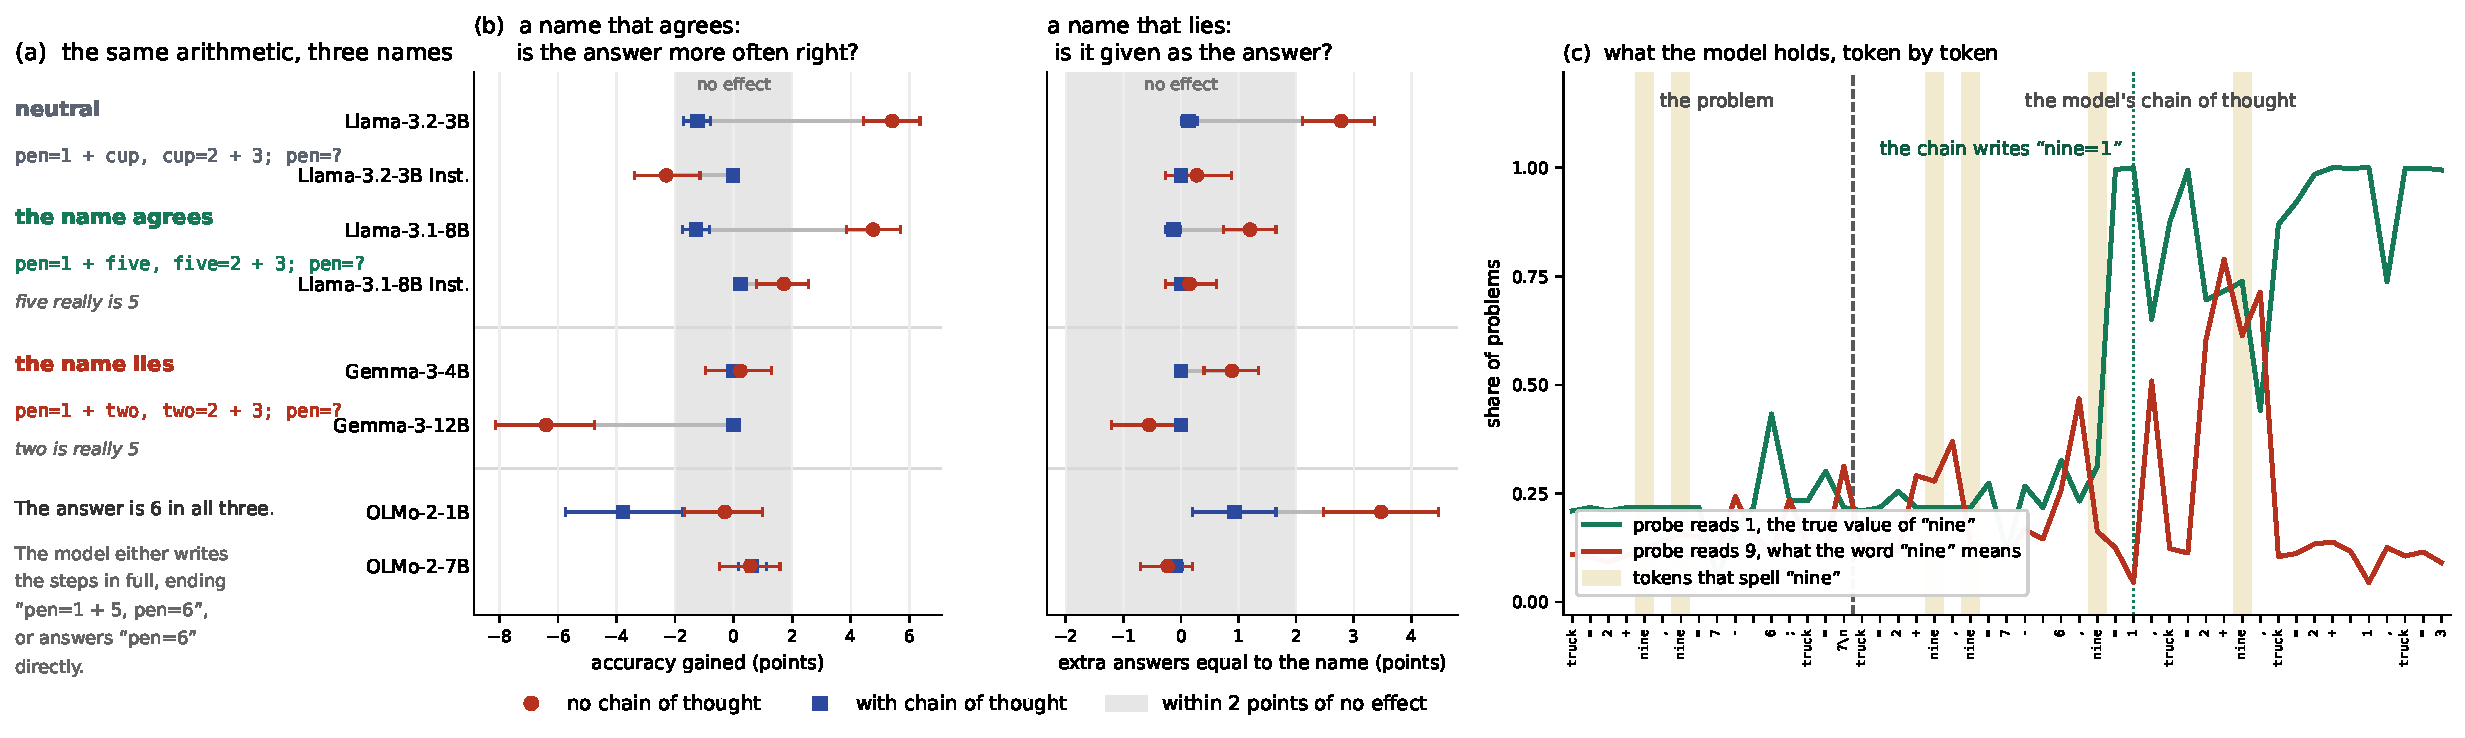
\includegraphics[width=\linewidth,height=0.88\textheight,keepaspectratio]{figures/fig1_master_L3.pdf}
\caption{Figure~1 at full size.}\label{fig:dump-fig1-master-L3}
\end{figure}
\end{landscape}

\begin{landscape}
\begin{figure}[p]\centering
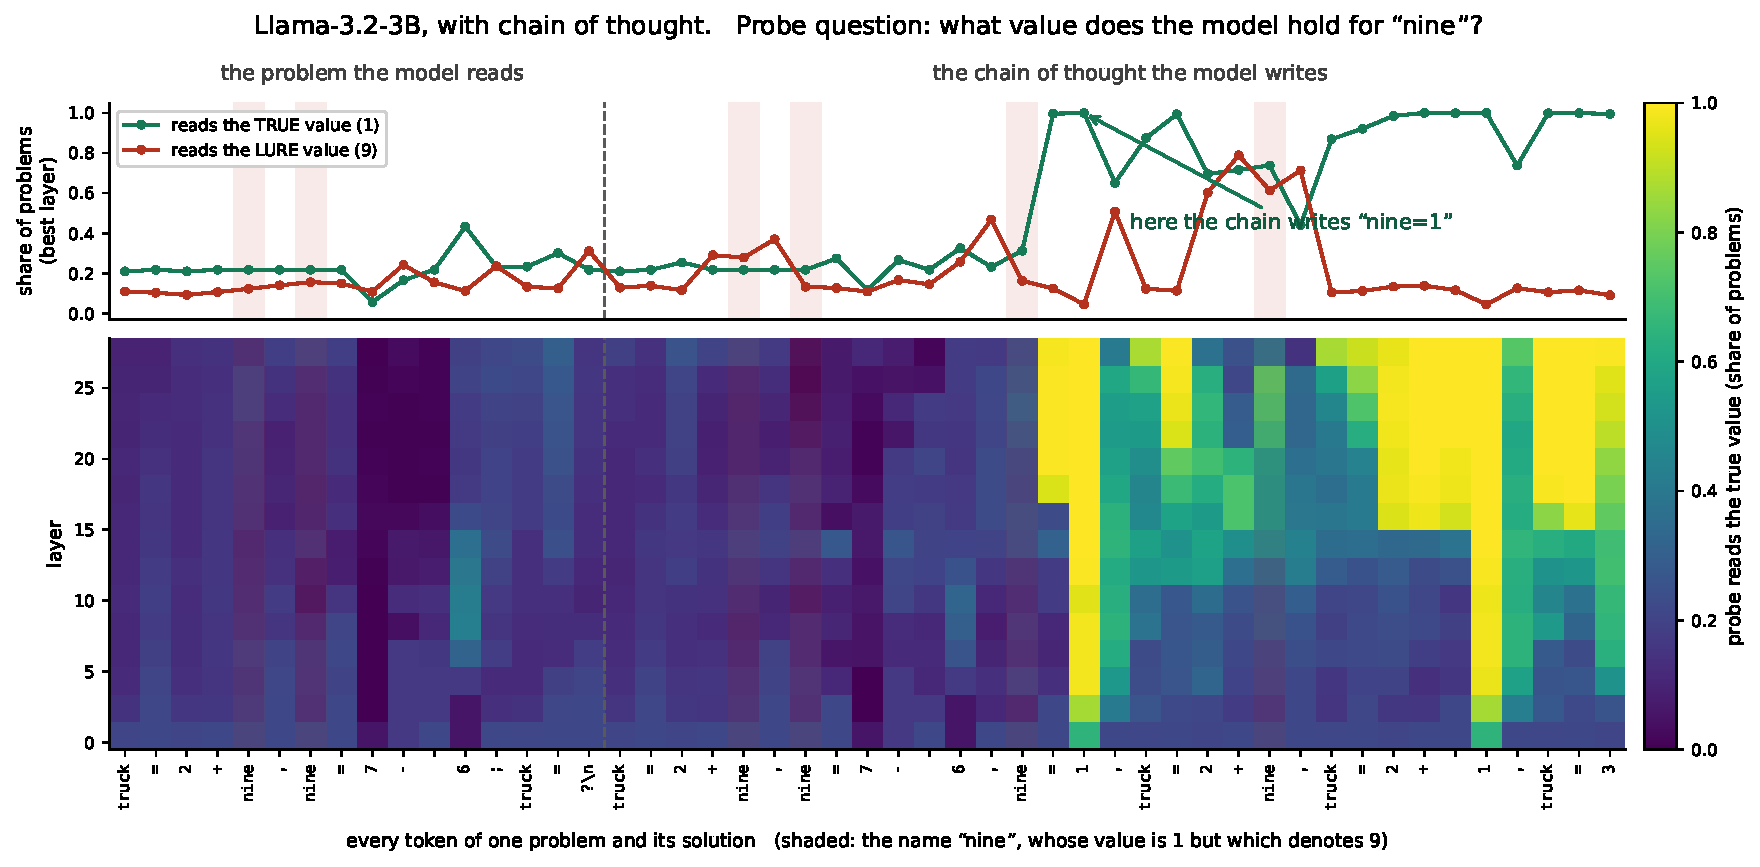
\includegraphics[width=\linewidth,height=0.88\textheight,keepaspectratio]{figures/fig2_tokens_llama32-3b_L3_cot_v2.pdf}
\caption{Figure~2 at full size: per-token probes, chain-of-thought regime, intermediate variable.}\label{fig:dump-fig2-tokens-llama32-3b-L3-cot-v2}
\end{figure}
\end{landscape}

\begin{landscape}
\begin{figure}[p]\centering
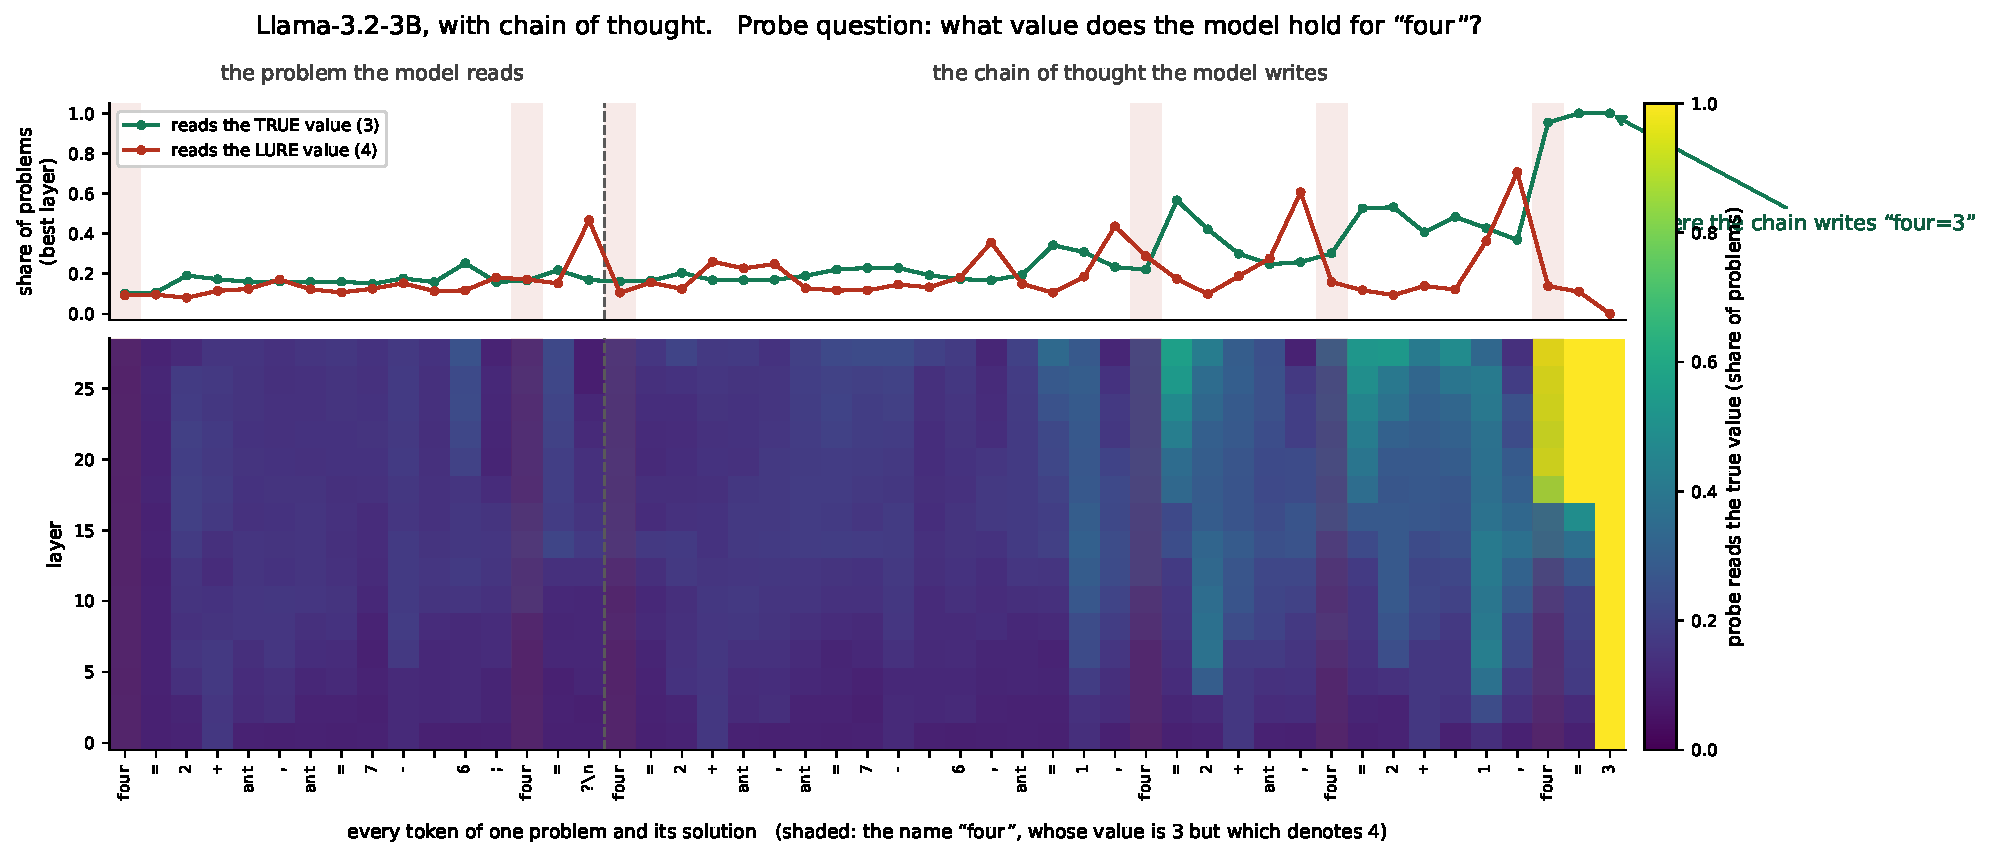
\includegraphics[width=\linewidth,height=0.88\textheight,keepaspectratio]{figures/fig2_tokens_llama32-3b_L3_cot_v1.pdf}
\caption{Per-token probes, chain-of-thought regime, queried variable.}\label{fig:dump-fig2-tokens-llama32-3b-L3-cot-v1}
\end{figure}
\end{landscape}

\begin{landscape}
\begin{figure}[p]\centering
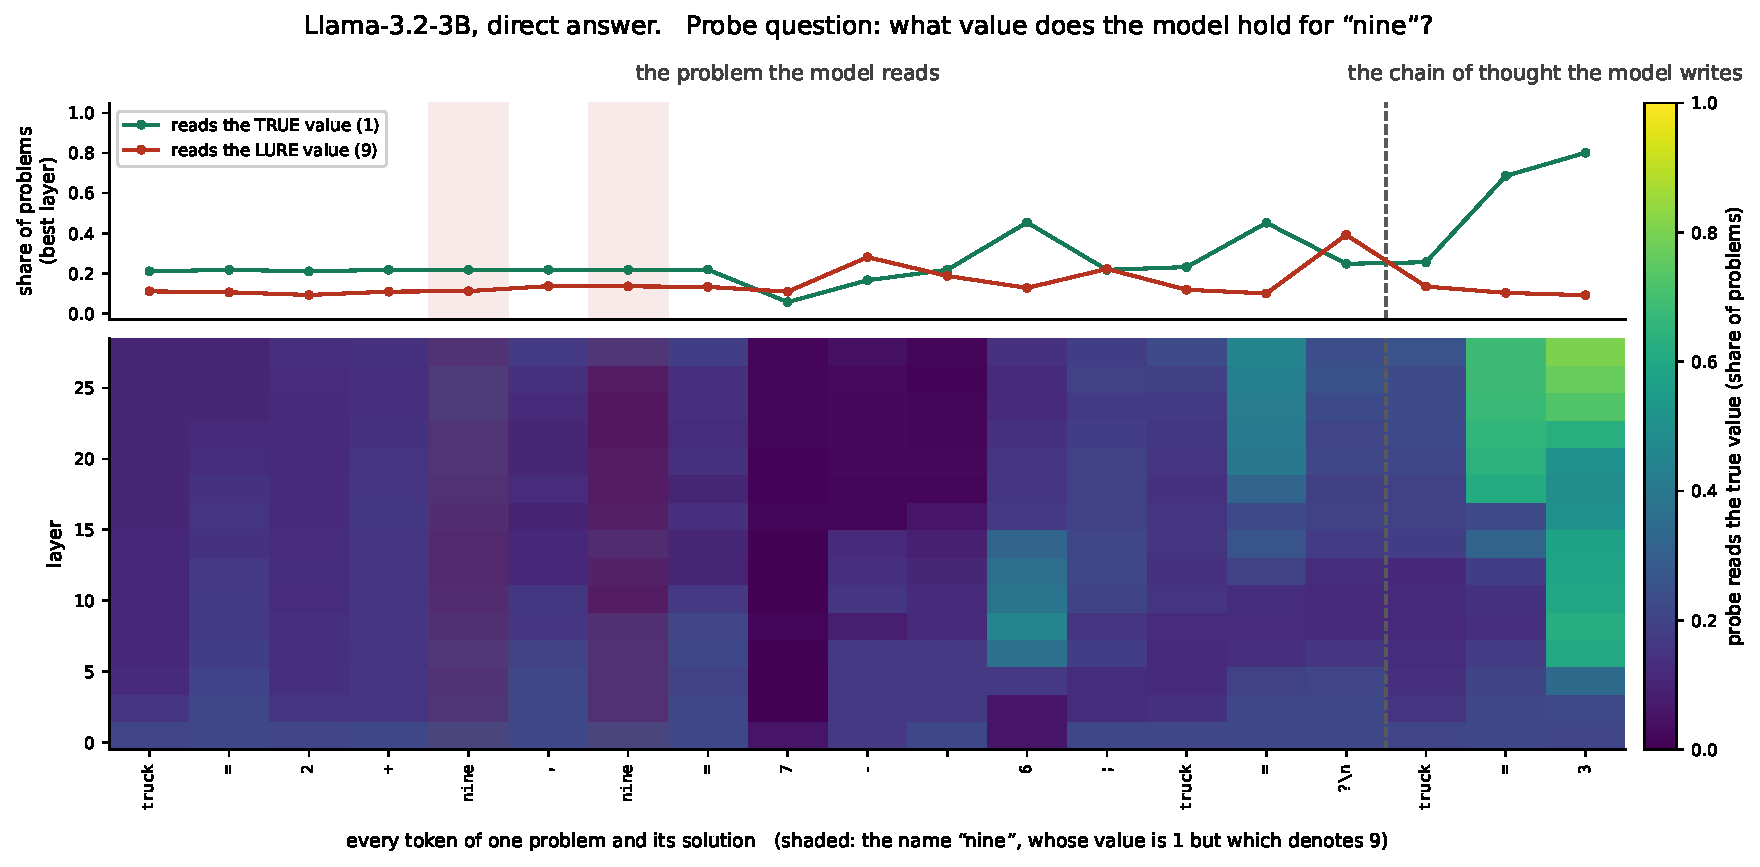
\includegraphics[width=\linewidth,height=0.88\textheight,keepaspectratio]{figures/fig2_tokens_llama32-3b_L3_direct_v2.pdf}
\caption{Per-token probes, direct regime, intermediate variable.}\label{fig:dump-fig2-tokens-llama32-3b-L3-direct-v2}
\end{figure}
\end{landscape}

\begin{landscape}
\begin{figure}[p]\centering
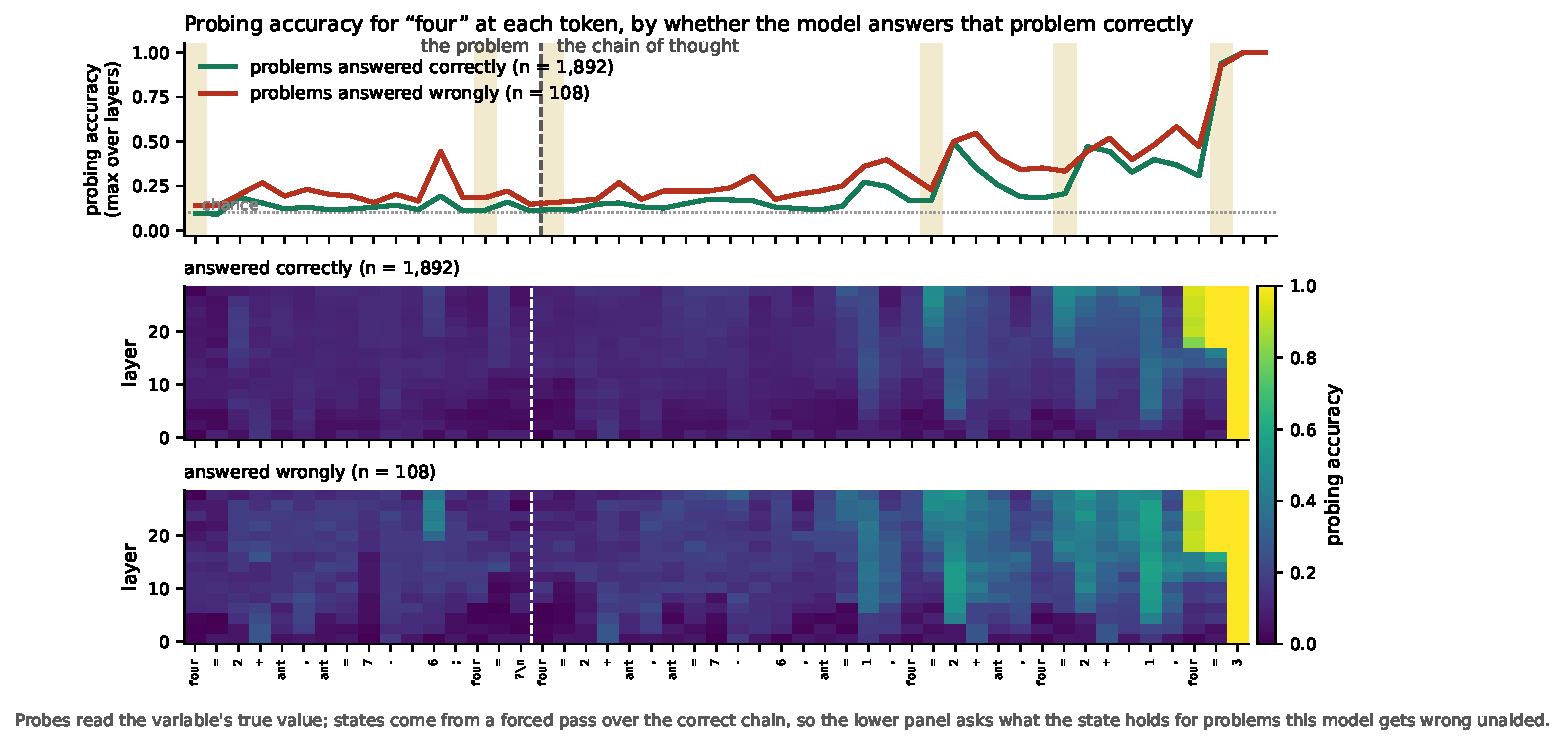
\includegraphics[width=\linewidth,height=0.88\textheight,keepaspectratio]{figures/fig4_errors_llama32-3b_L3_cot_v1.pdf}
\caption{Probing accuracy split by whether the model answers the problem correctly on its own, with the layer sweep for each half.}\label{fig:dump-fig4-errors-llama32-3b-L3-cot-v1}
\end{figure}
\end{landscape}

\begin{landscape}
\begin{figure}[p]\centering
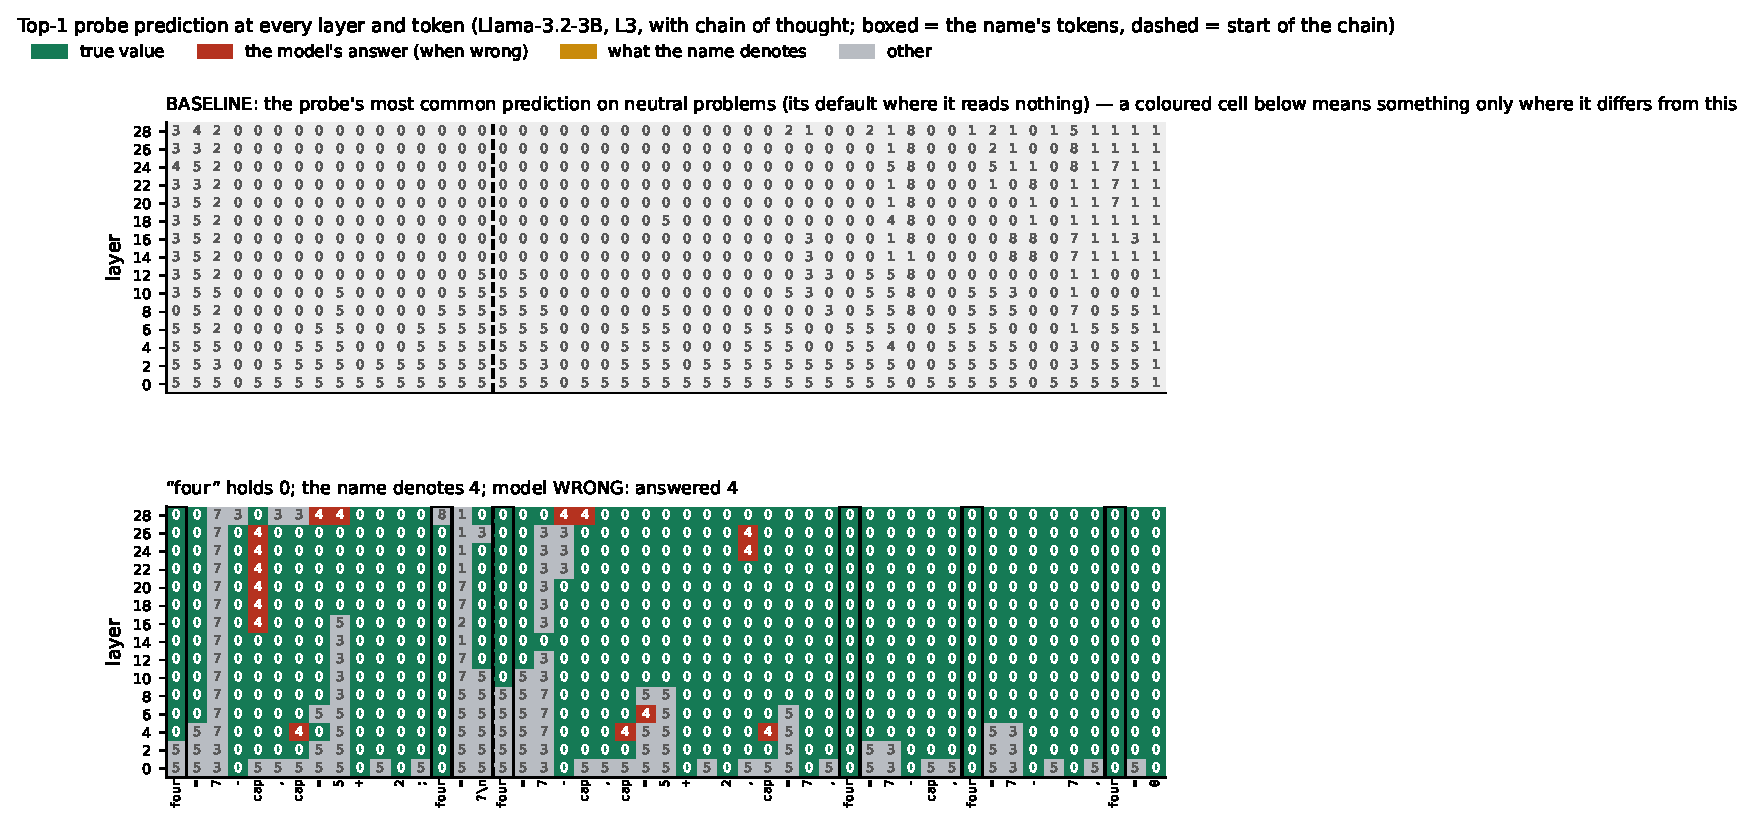
\includegraphics[width=\linewidth,height=0.88\textheight,keepaspectratio]{figures/fig5_kudo3_llama32-3b_L3_cot_v1_lureerr_i0.pdf}
\caption{Top-1 probe prediction at every layer and token, on a problem answered with the lure. Layout after \citeauthor{kudo2026faithful}'s Figure~3.}\label{fig:dump-fig5-kudo3-llama32-3b-L3-cot-v1-lureerr-i0}
\end{figure}
\end{landscape}

\begin{landscape}
\begin{figure}[p]\centering
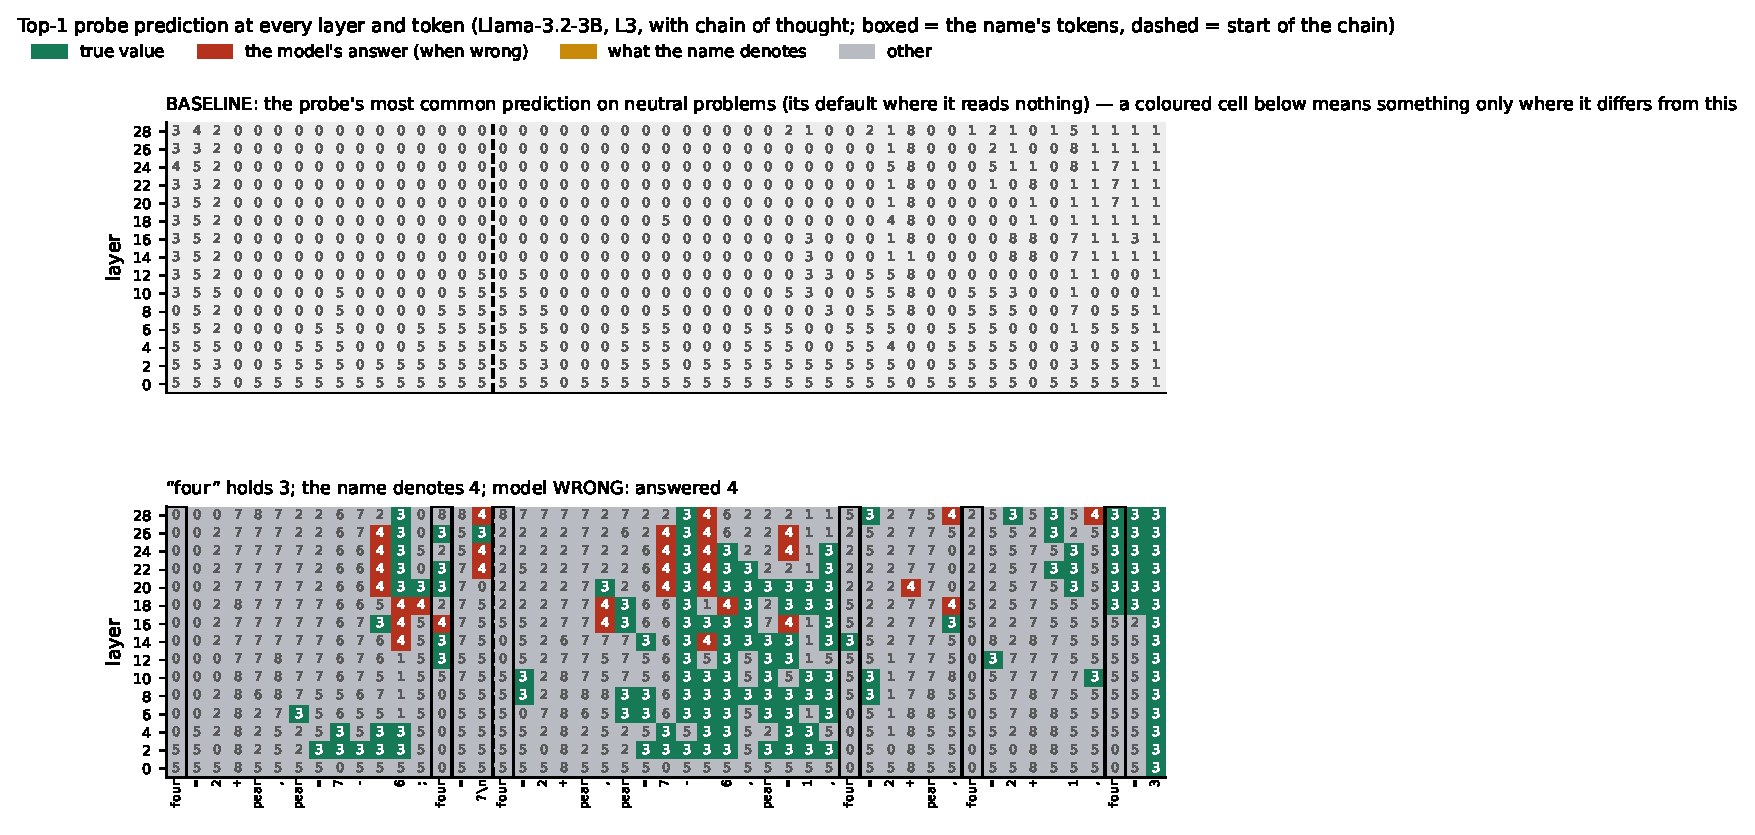
\includegraphics[width=\linewidth,height=0.88\textheight,keepaspectratio]{figures/fig5_kudo3_llama32-3b_L3_cot_v1_lureerr_i1.pdf}
\caption{A second problem answered with the lure.}\label{fig:dump-fig5-kudo3-llama32-3b-L3-cot-v1-lureerr-i1}
\end{figure}
\end{landscape}

\begin{landscape}
\begin{figure}[p]\centering
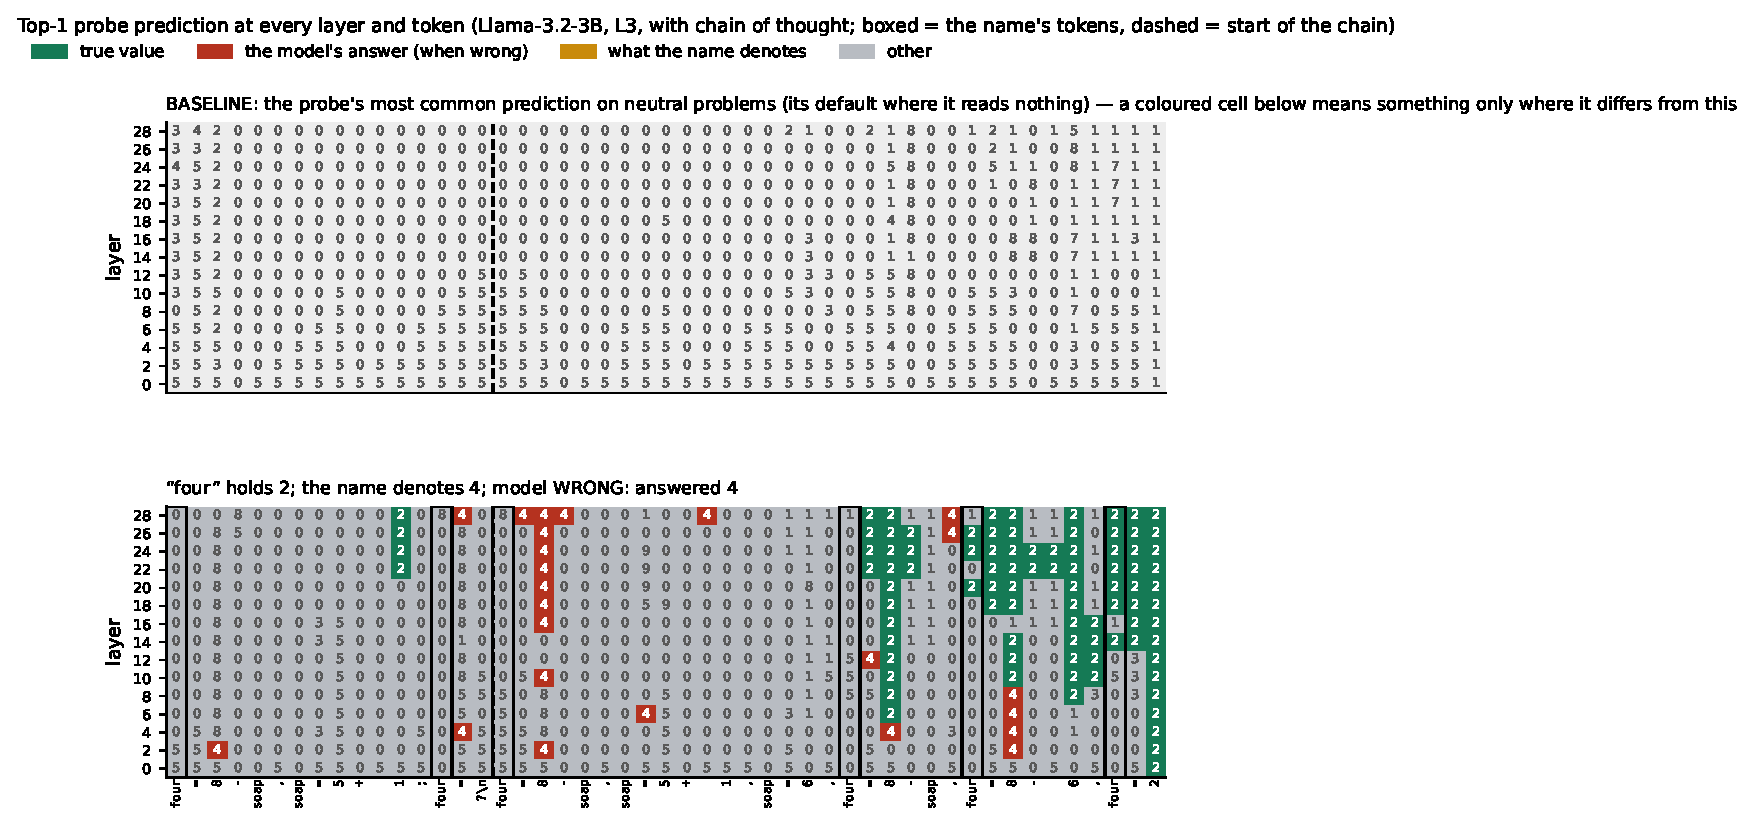
\includegraphics[width=\linewidth,height=0.88\textheight,keepaspectratio]{figures/fig5_kudo3_llama32-3b_L3_cot_v1_lureerr_i2.pdf}
\caption{A third problem answered with the lure.}\label{fig:dump-fig5-kudo3-llama32-3b-L3-cot-v1-lureerr-i2}
\end{figure}
\end{landscape}

\begin{landscape}
\begin{figure}[p]\centering
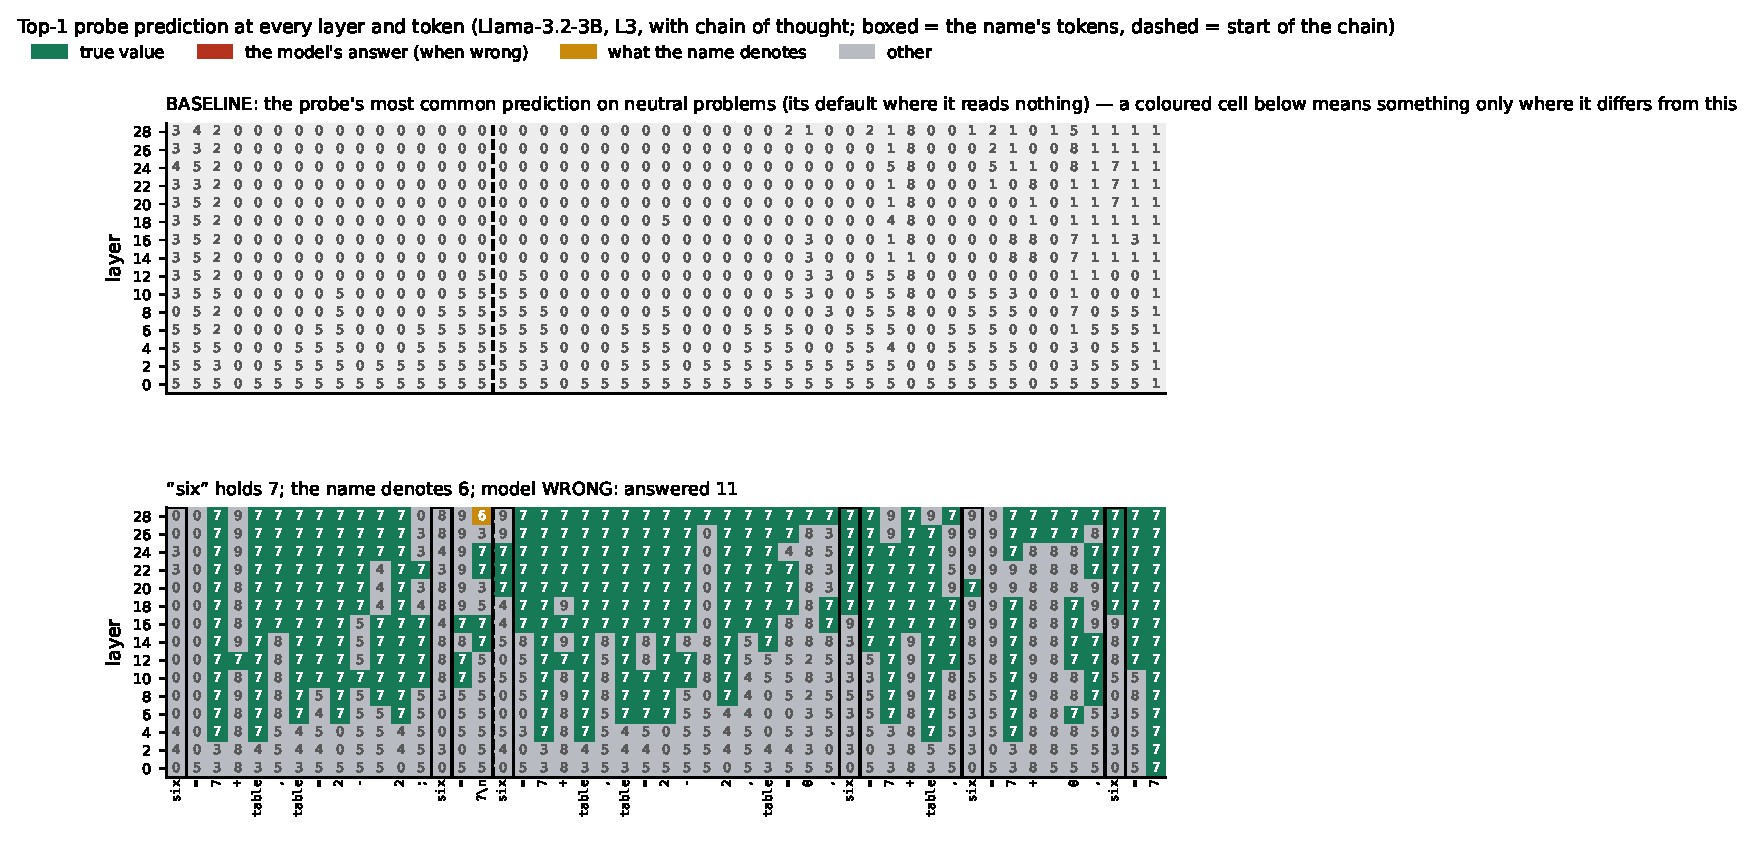
\includegraphics[width=\linewidth,height=0.88\textheight,keepaspectratio]{figures/fig5_kudo3_llama32-3b_L3_cot_v1_err_i0.pdf}
\caption{As above, on a problem answered wrongly for another reason.}\label{fig:dump-fig5-kudo3-llama32-3b-L3-cot-v1-err-i0}
\end{figure}
\end{landscape}

\begin{landscape}
\begin{figure}[p]\centering
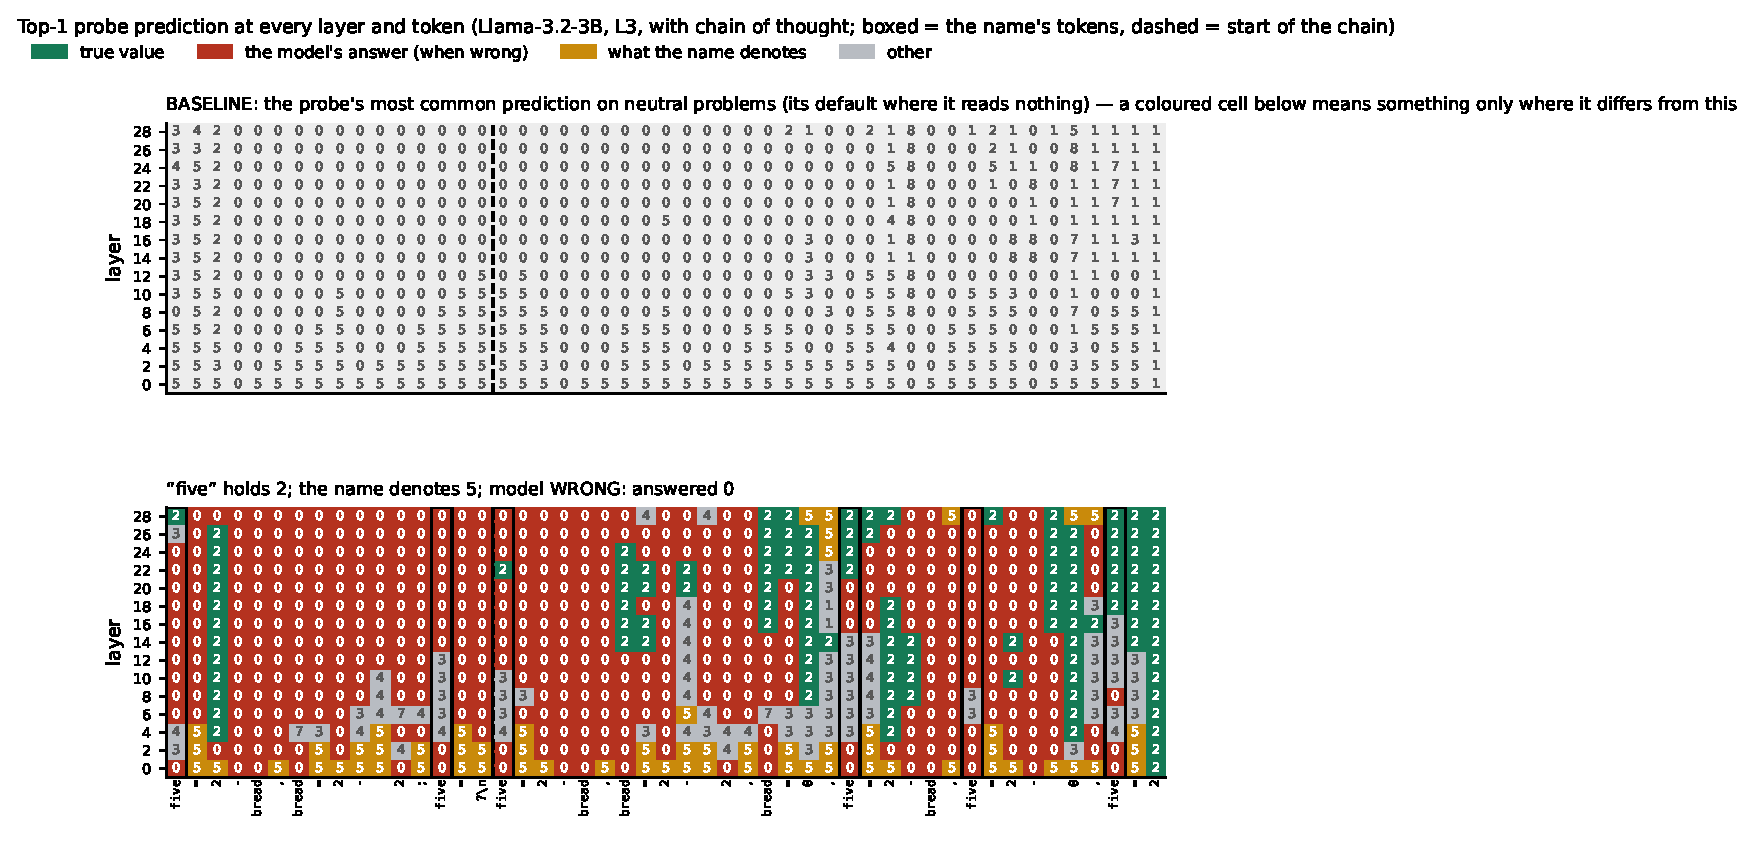
\includegraphics[width=\linewidth,height=0.88\textheight,keepaspectratio]{figures/fig5_kudo3_llama32-3b_L3_cot_v1_err_i1.pdf}
\caption{A second such problem.}\label{fig:dump-fig5-kudo3-llama32-3b-L3-cot-v1-err-i1}
\end{figure}
\end{landscape}

\begin{landscape}
\begin{figure}[p]\centering
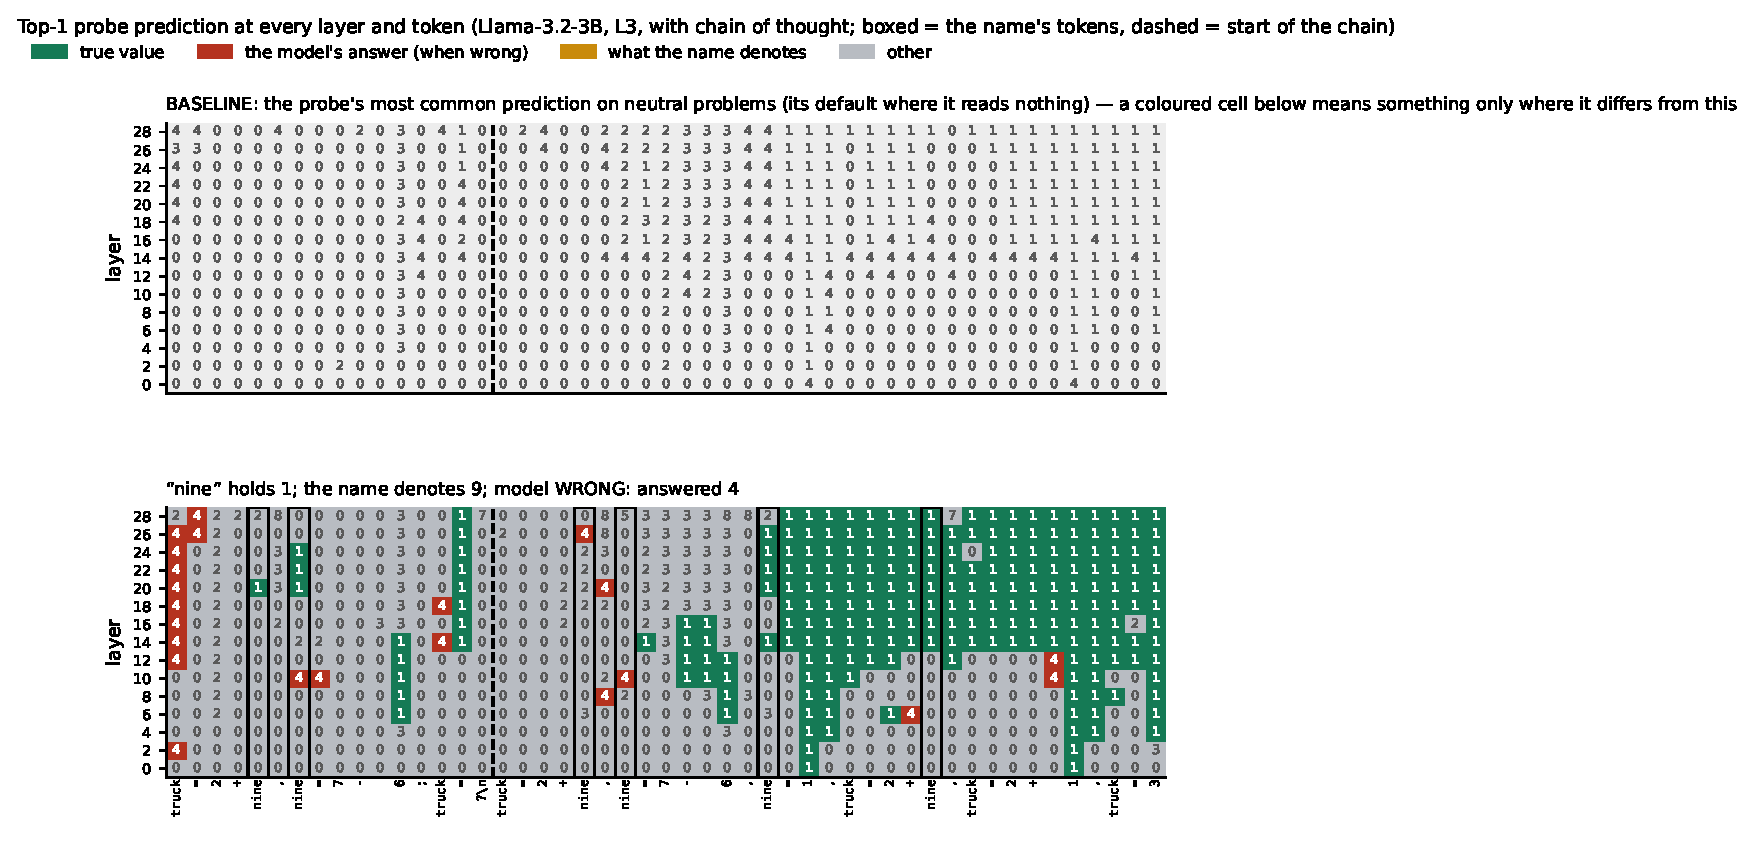
\includegraphics[width=\linewidth,height=0.88\textheight,keepaspectratio]{figures/fig5_kudo3_llama32-3b_L3_cot_v2_err_i0.pdf}
\caption{As above, for the intermediate variable.}\label{fig:dump-fig5-kudo3-llama32-3b-L3-cot-v2-err-i0}
\end{figure}
\end{landscape}

\begin{landscape}
\begin{figure}[p]\centering
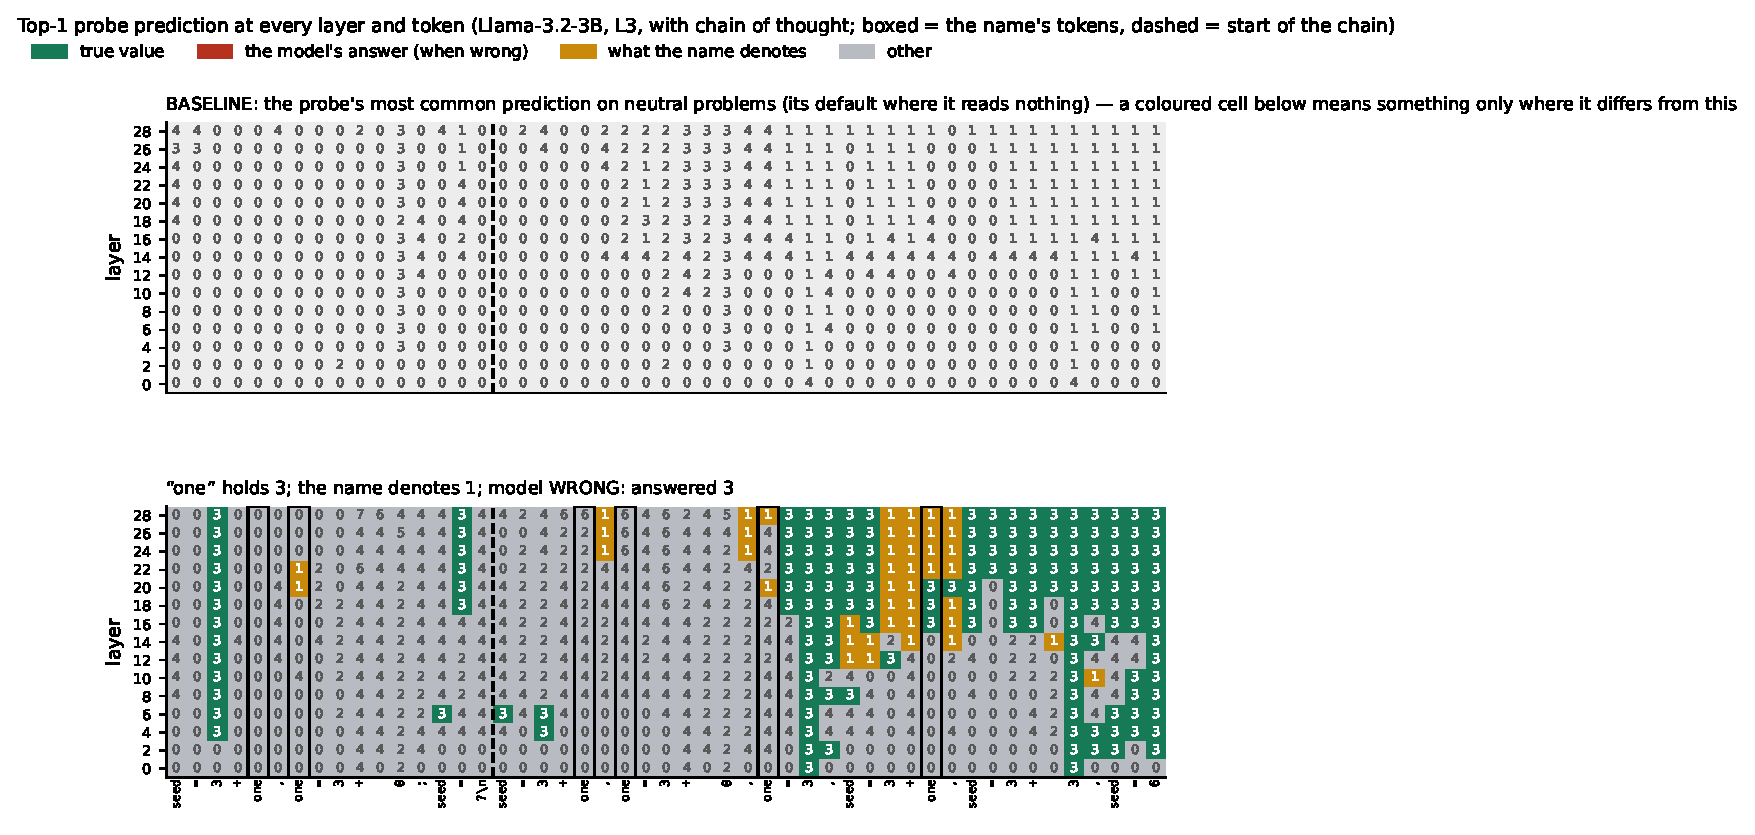
\includegraphics[width=\linewidth,height=0.88\textheight,keepaspectratio]{figures/fig5_kudo3_llama32-3b_L3_cot_v2_err_i1.pdf}
\caption{A second problem, intermediate variable.}\label{fig:dump-fig5-kudo3-llama32-3b-L3-cot-v2-err-i1}
\end{figure}
\end{landscape}

\begin{landscape}
\begin{figure}[p]\centering
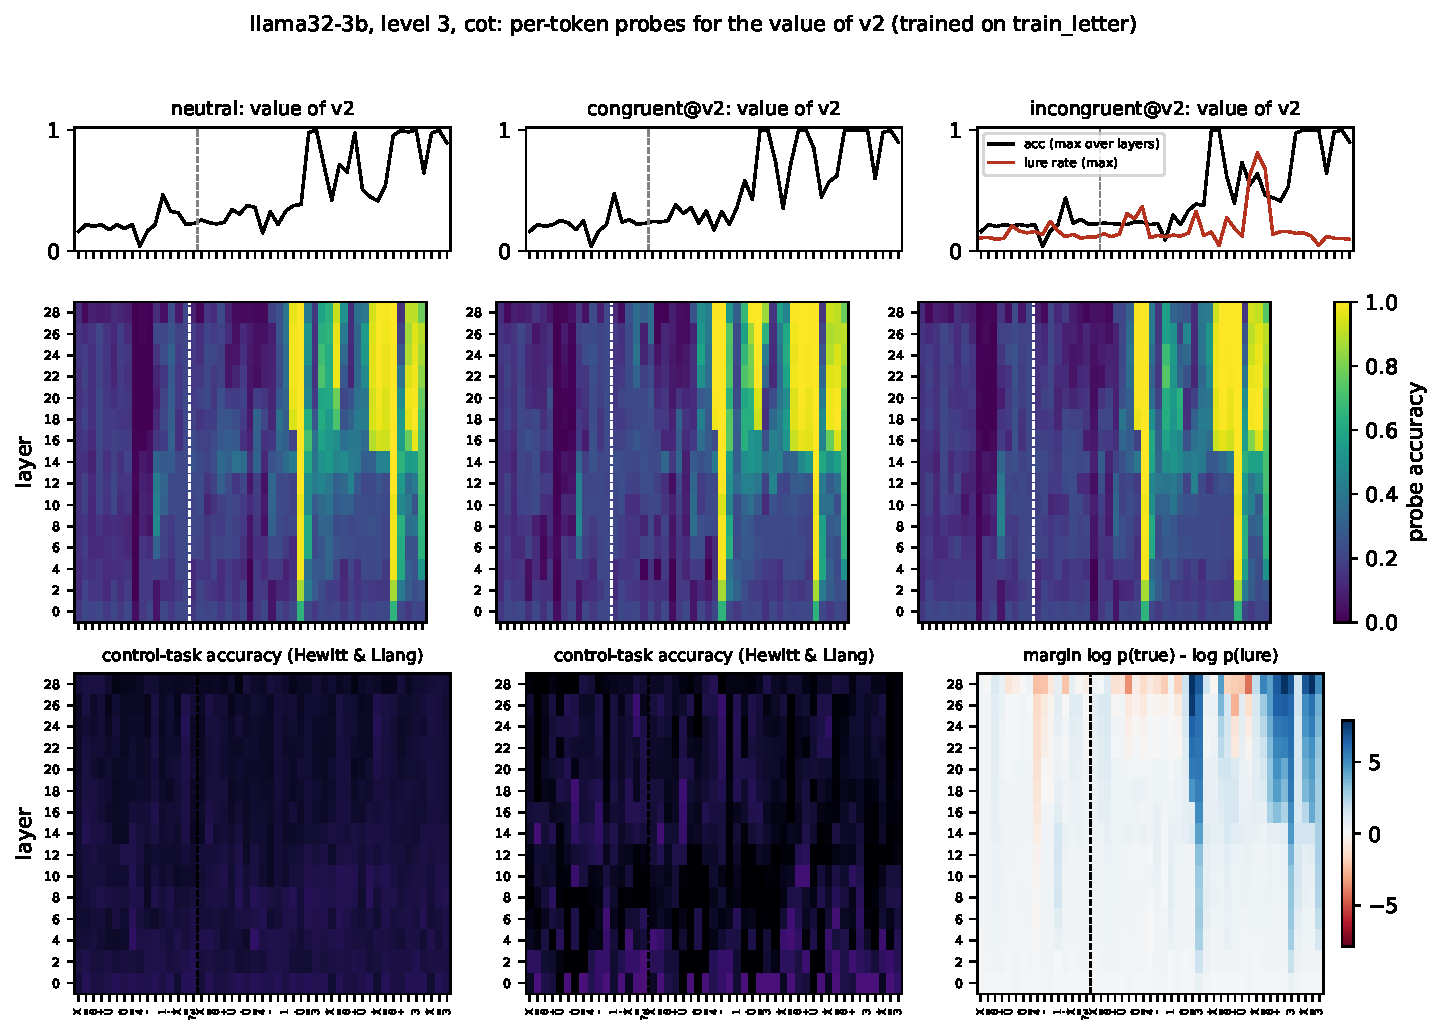
\includegraphics[width=\linewidth,height=0.88\textheight,keepaspectratio]{figures/kudo_fig2_llama32-3b_L3_cot_v2.pdf}
\caption{Accuracy heatmaps by token and layer for the neutral, congruent and incongruent conditions, in the layout of \citeauthor{kudo2026faithful}'s Figure~2.}\label{fig:dump-kudo-fig2-llama32-3b-L3-cot-v2}
\end{figure}
\end{landscape}

\begin{landscape}
\begin{figure}[p]\centering
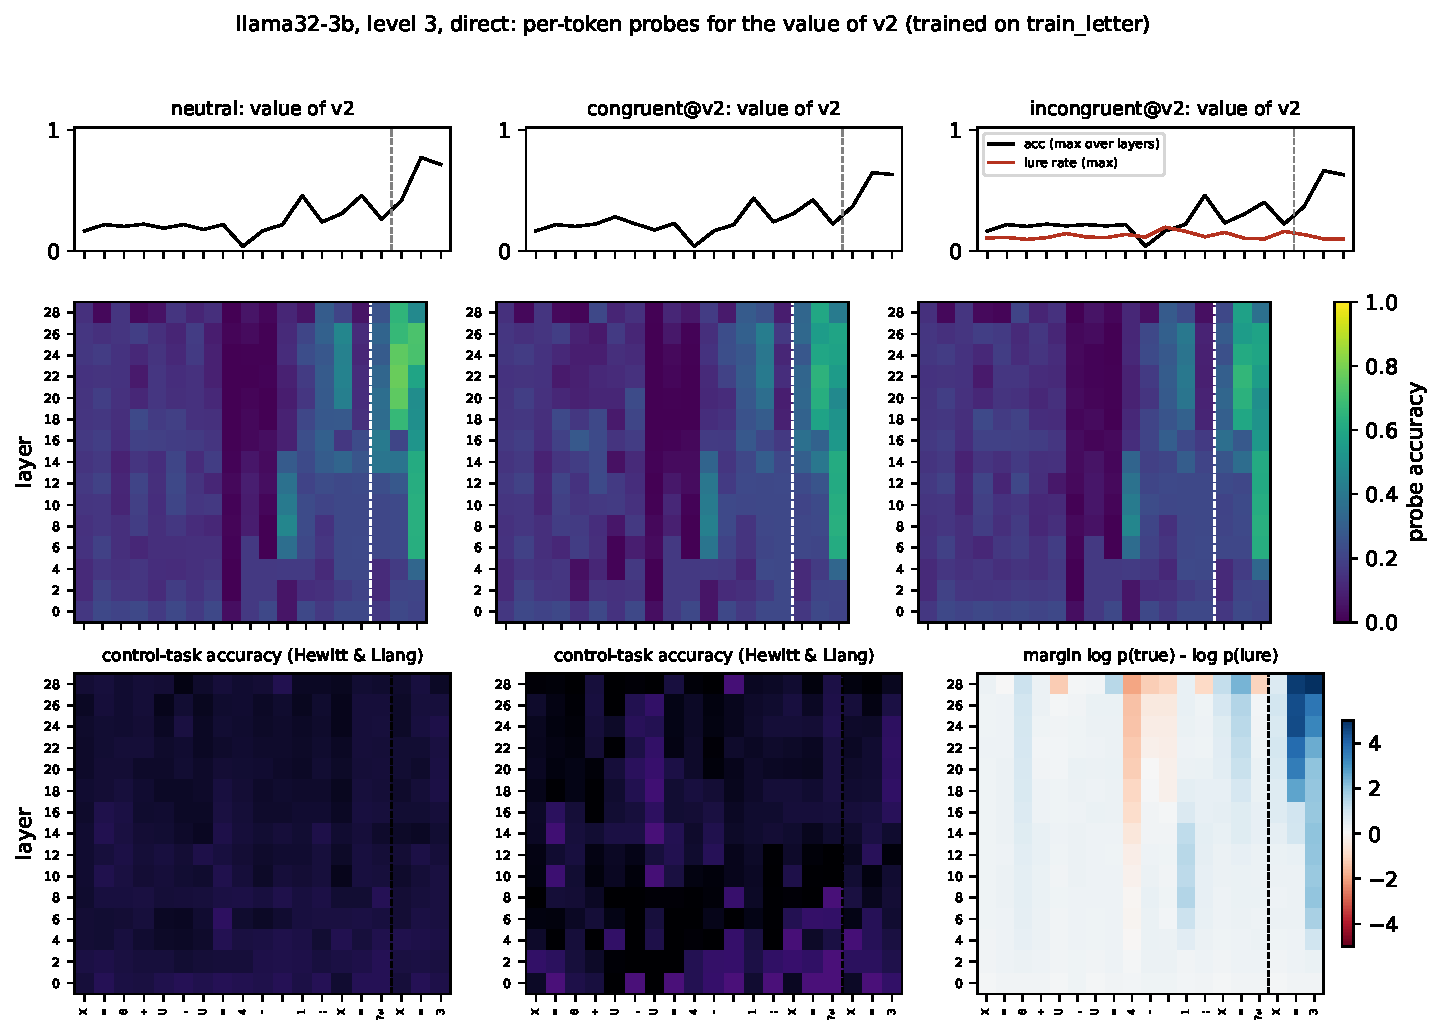
\includegraphics[width=\linewidth,height=0.88\textheight,keepaspectratio]{figures/kudo_fig2_llama32-3b_L3_direct_v2.pdf}
\caption{The same heatmaps in the direct regime.}\label{fig:dump-kudo-fig2-llama32-3b-L3-direct-v2}
\end{figure}
\end{landscape}

\begin{landscape}
\begin{figure}[p]\centering
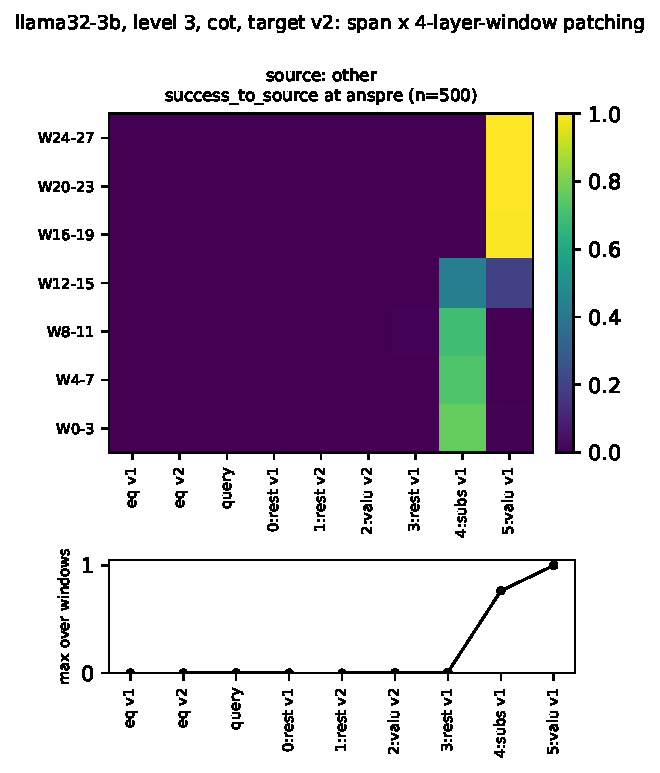
\includegraphics[width=\linewidth,height=0.88\textheight,keepaspectratio]{figures/kudo_fig5_llama32-3b_L3_cot_v2.pdf}
\caption{Span-by-layer-window patching grids, three sources, after \citeauthor{kudo2026faithful}'s Figures~5--6.}\label{fig:dump-kudo-fig5-llama32-3b-L3-cot-v2}
\end{figure}
\end{landscape}

\begin{landscape}
\begin{figure}[p]\centering
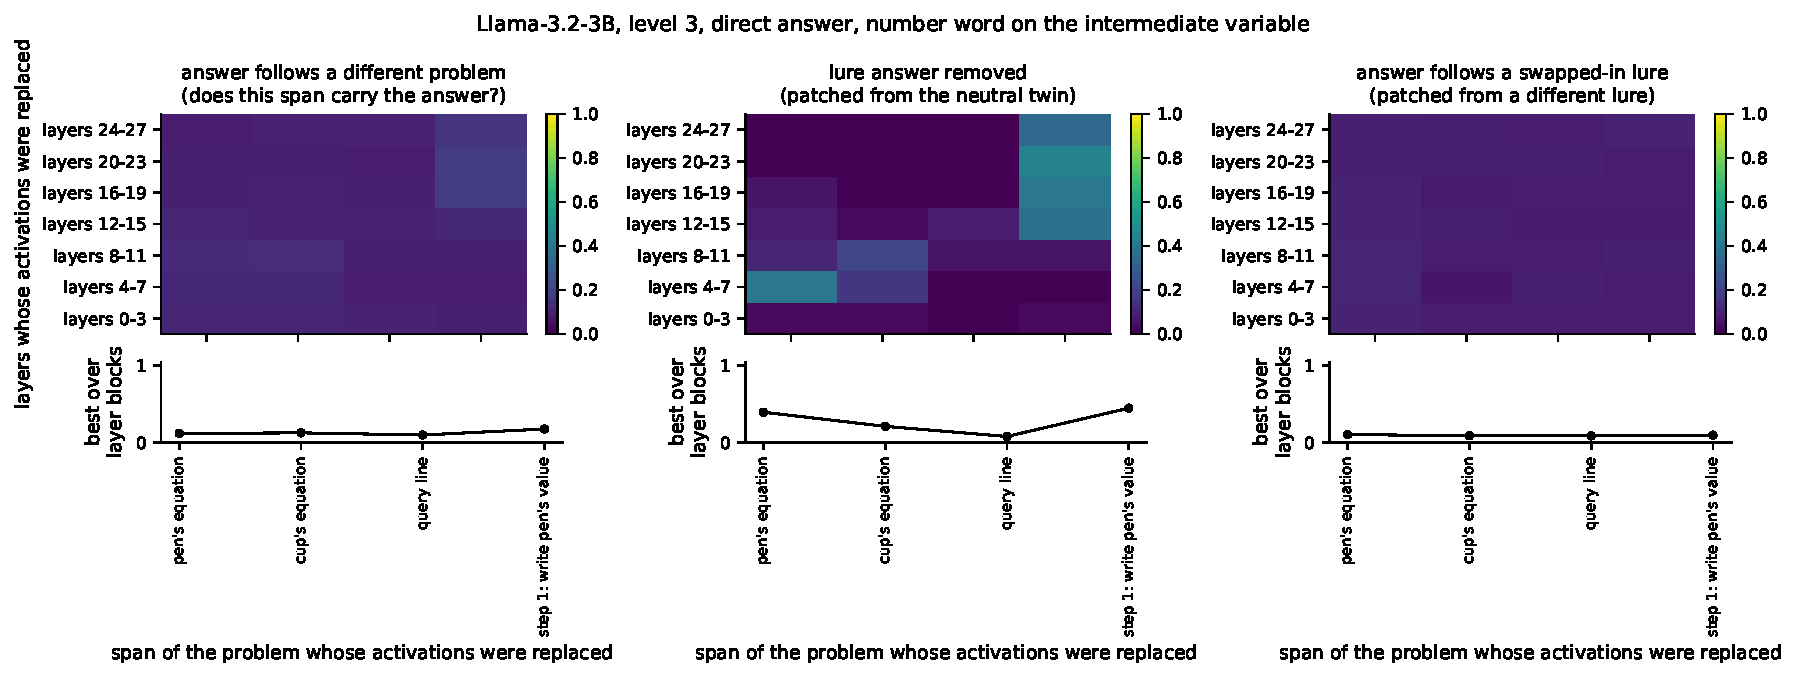
\includegraphics[width=\linewidth,height=0.88\textheight,keepaspectratio]{figures/kudo_fig5_llama32-3b_L3_direct_v2.pdf}
\caption{The same grids in the direct regime.}\label{fig:dump-kudo-fig5-llama32-3b-L3-direct-v2}
\end{figure}
\end{landscape}

\begin{landscape}
\begin{figure}[p]\centering
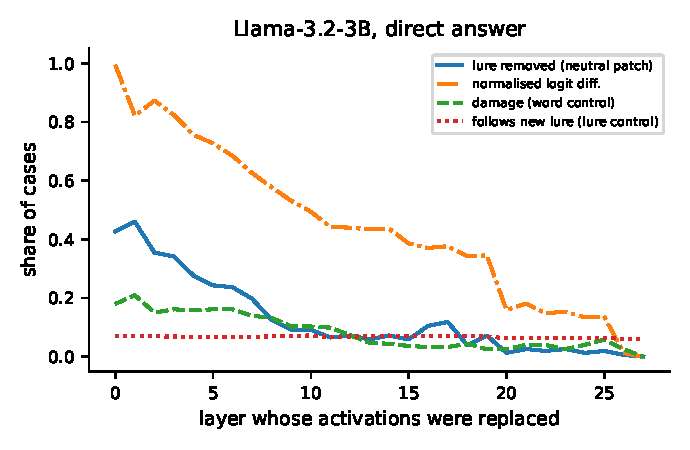
\includegraphics[width=\linewidth,height=0.88\textheight,keepaspectratio]{figures/fig3_patching_llama32-3b_L3_v2.pdf}
\caption{Lure errors removed by patching, by layer, with both controls.}\label{fig:dump-fig3-patching-llama32-3b-L3-v2}
\end{figure}
\end{landscape}

\begin{landscape}
\begin{figure}[p]\centering
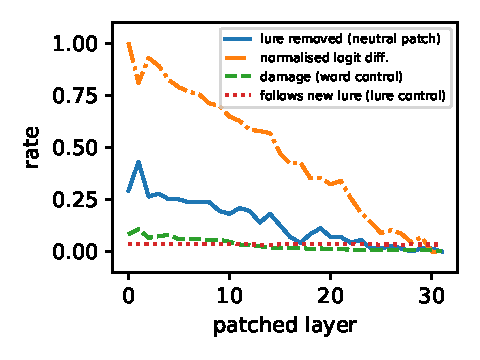
\includegraphics[width=\linewidth,height=0.88\textheight,keepaspectratio]{figures/fig3_patching_llama31-8b_L3_v2.pdf}
\caption{\texttt{fig3\_patching\_llama31-8b\_L3\_v2}.}\label{fig:dump-fig3-patching-llama31-8b-L3-v2}
\end{figure}
\end{landscape}

\begin{landscape}
\begin{figure}[p]\centering
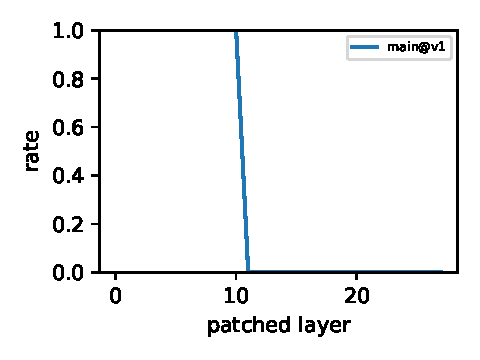
\includegraphics[width=\linewidth,height=0.88\textheight,keepaspectratio]{figures/fig3_patching_llama32-3b_L3_v1.pdf}
\caption{\texttt{fig3\_patching\_llama32-3b\_L3\_v1}.}\label{fig:dump-fig3-patching-llama32-3b-L3-v1}
\end{figure}
\end{landscape}

\begin{landscape}
\begin{figure}[p]\centering
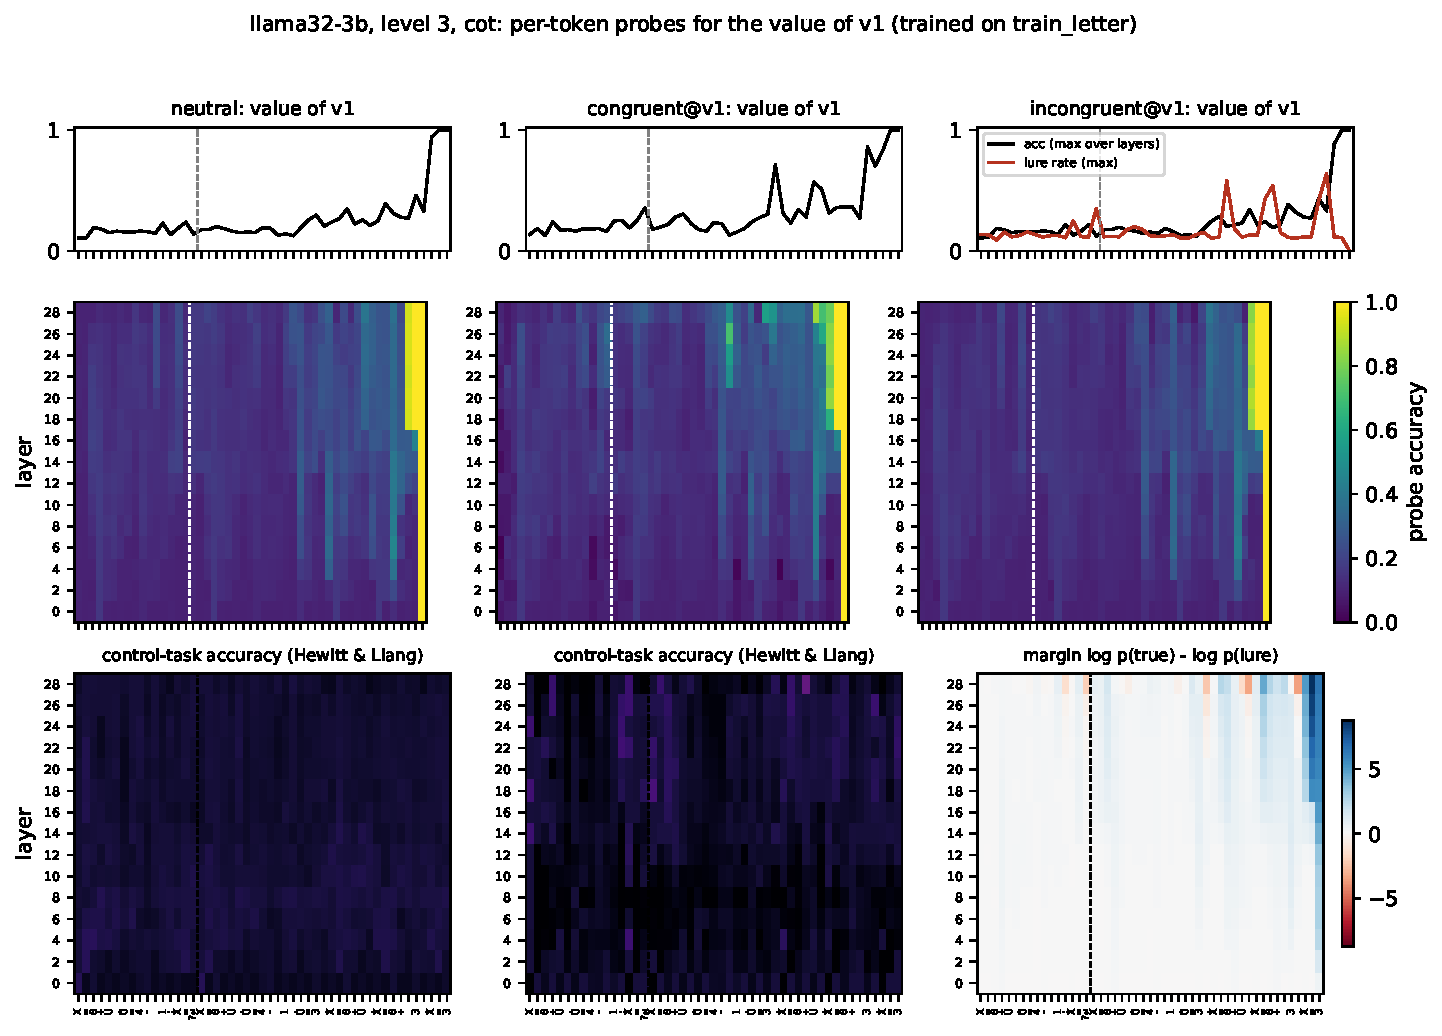
\includegraphics[width=\linewidth,height=0.88\textheight,keepaspectratio]{figures/kudo_fig2_llama32-3b_L3_cot_v1.pdf}
\caption{\texttt{kudo\_fig2\_llama32-3b\_L3\_cot\_v1}.}\label{fig:dump-kudo-fig2-llama32-3b-L3-cot-v1}
\end{figure}
\end{landscape}

\begin{landscape}
\begin{figure}[p]\centering
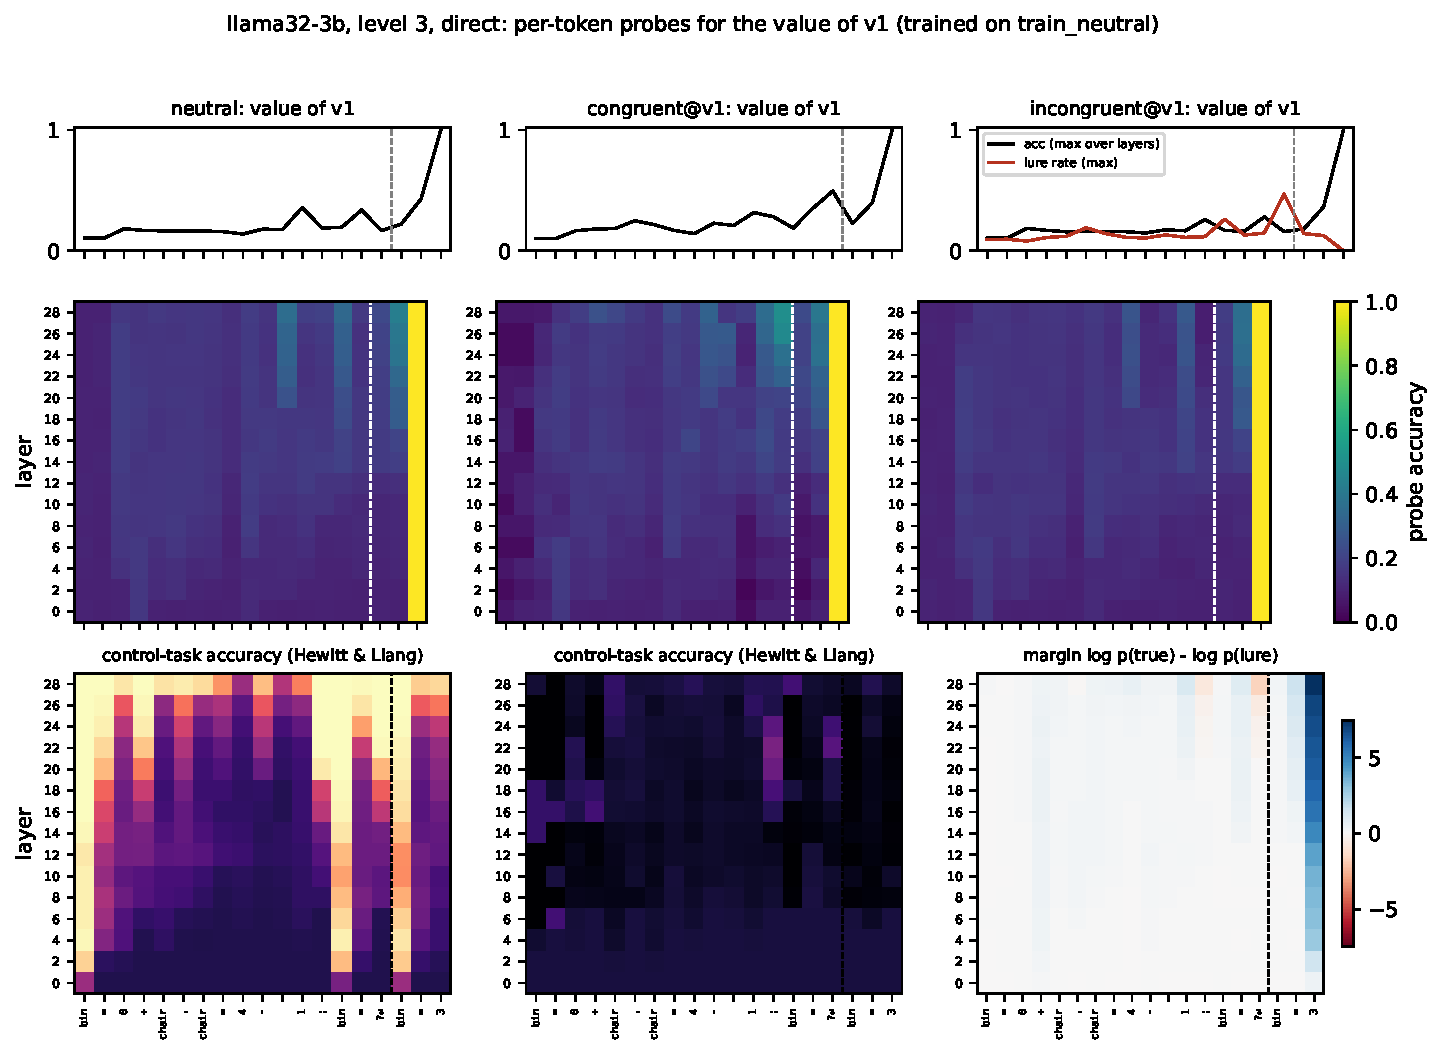
\includegraphics[width=\linewidth,height=0.88\textheight,keepaspectratio]{figures/kudo_fig2_llama32-3b_L3_direct_v1.pdf}
\caption{\texttt{kudo\_fig2\_llama32-3b\_L3\_direct\_v1}.}\label{fig:dump-kudo-fig2-llama32-3b-L3-direct-v1}
\end{figure}
\end{landscape}

\begin{landscape}
\begin{figure}[p]\centering
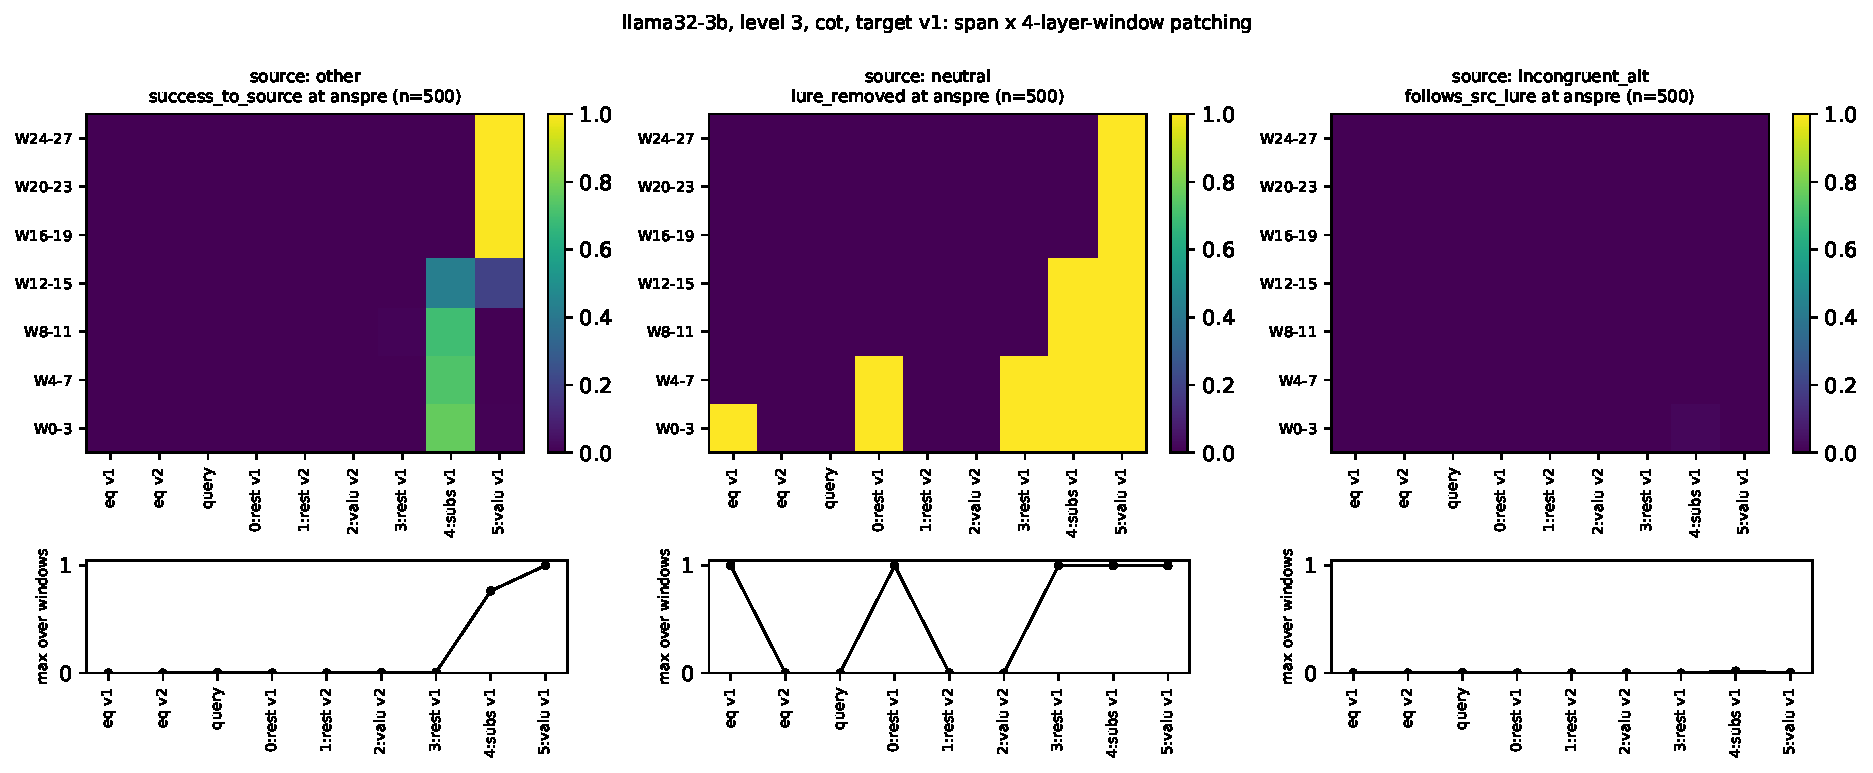
\includegraphics[width=\linewidth,height=0.88\textheight,keepaspectratio]{figures/kudo_fig5_llama32-3b_L3_cot_v1.pdf}
\caption{\texttt{kudo\_fig5\_llama32-3b\_L3\_cot\_v1}.}\label{fig:dump-kudo-fig5-llama32-3b-L3-cot-v1}
\end{figure}
\end{landscape}

\begin{landscape}
\begin{figure}[p]\centering
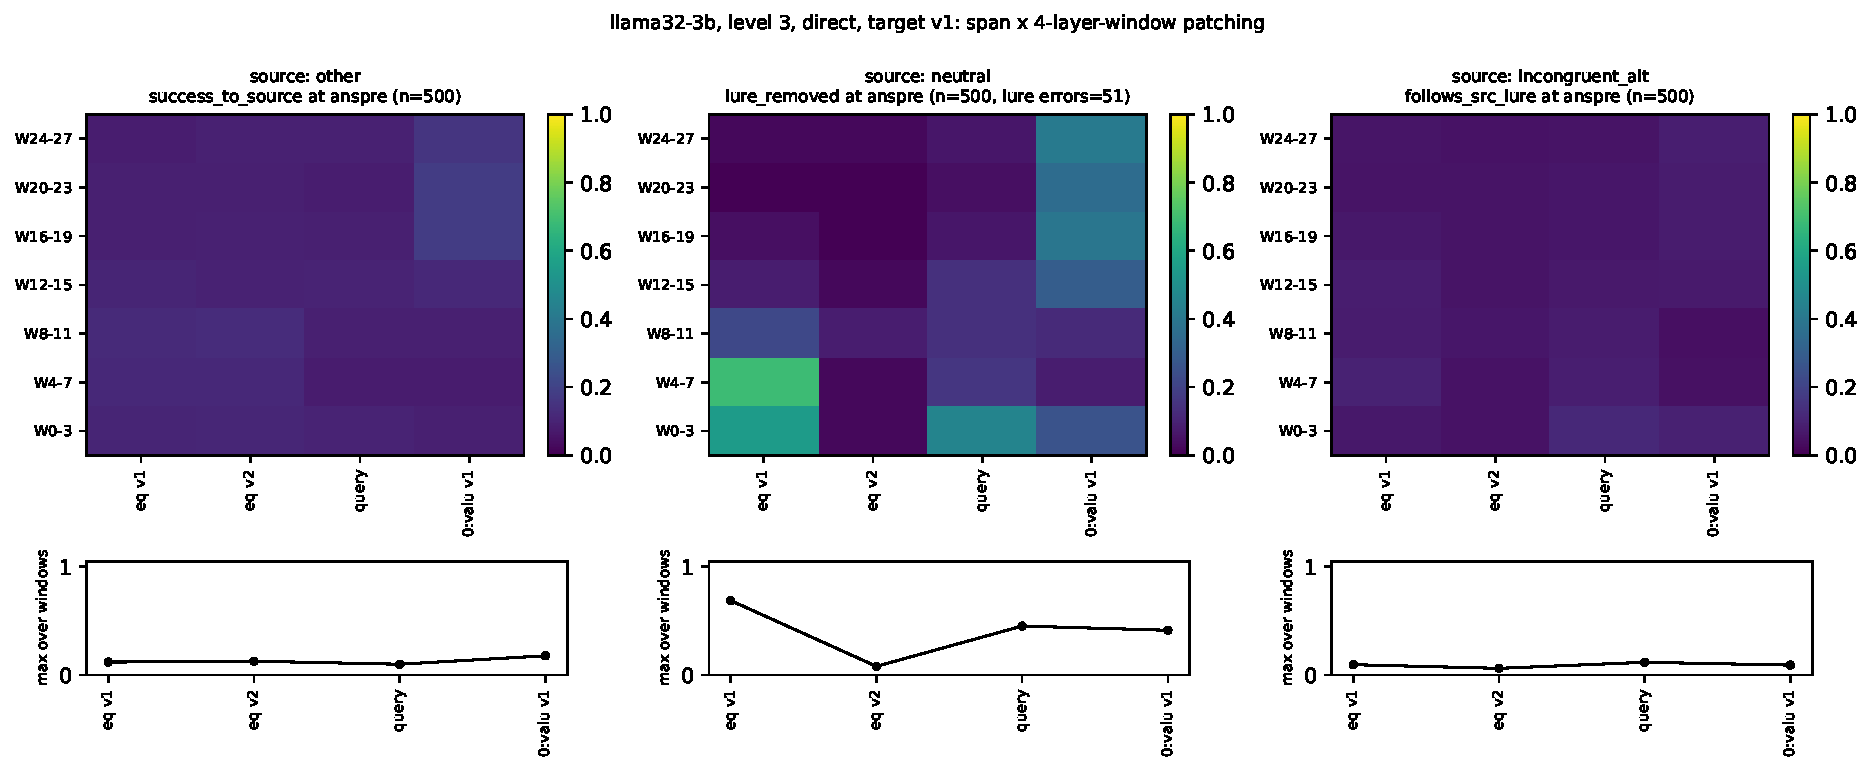
\includegraphics[width=\linewidth,height=0.88\textheight,keepaspectratio]{figures/kudo_fig5_llama32-3b_L3_direct_v1.pdf}
\caption{\texttt{kudo\_fig5\_llama32-3b\_L3\_direct\_v1}.}\label{fig:dump-kudo-fig5-llama32-3b-L3-direct-v1}
\end{figure}
\end{landscape}
